\PassOptionsToPackage{table}{xcolor}
%\documentclass{beamer}
\documentclass[compress]{beamer}
%\usetheme{Epam}
\usetheme{Copenhagen}
\usepackage{xcolor}
\usepackage{listings}
\usepackage{graphicx}
\usepackage[utf8]{inputenc}
\usepackage{datetime}
\usepackage{beamerthemesplit}
%\beamertemplatenavigationsymbolsempty
\usepackage{listingsutf8}
\usepackage{ragged2e}
\usepackage{hyperref}
\lstset{ %
  language=C,                      % the language of the code
%  basicstyle=\ttfamily,           % the size of the fonts that are used for the code
%  basicstyle=\ttfamily\tiny,      % the size of the fonts that are used for the code
  basicstyle=\ttfamily\scriptsize, % the size of the fonts that are used for the code
  numbers=left,                    % where to put the line-numbers
  numberstyle=\tiny\color{gray},   % the style that is used for the line-numbers
  stepnumber=1,                    % the step between two line-numbers. If it's 1, each line 
                                   % will be numbered
  numbersep=5pt,                   % how far the line-numbers are from the code
  %backgroundcolor=\color{gray},   % choose the background color. You must add \usepackage{color}
  showspaces=false,               % show spaces adding particular underscores
  showstringspaces=false,         % underline spaces within strings
  showtabs=false,                 % show tabs within strings adding particular underscores
%  frame=shadowbox,                   % adds a frame around the code
  rulecolor=\color{black},        % if not set, the frame-color may be changed on line-breaks within not-black text (e.g. commens (green here))
  tabsize=4,                      % sets default tabsize to 4 spaces
  captionpos=,                   % sets the caption-position to bottom
  breaklines=false,                % sets automatic line breaking
  breakatwhitespace=false,        % sets if automatic breaks should only happen at whitespace
  title=\lstname,                 % show the filename of files included with \lstinputlisting;
                                  % also try caption instead of title
  keywordstyle=\color{blue},      % keyword style
  commentstyle=\color{mygreen},   % comment style
  stringstyle=\color{magenta},    % string literal style
%  escapeinside={\%*}{*)},        % if you want to add a comment within your code
  inputencoding=utf8,
  extendedchars=\true,
  morekeywords={*,..., restrict, alignof, alignas, bool, true, false, size_t, ssize_t, inline, \_Noreturn, noreturn},
  breakautoindent=false,
  breakindent=1pt,
}

%\setbeameroption{show only notes}
%\usepackage{pgfpages}
%\setbeameroption{show notes}
%\setbeameroption{show notes on second screen=right}

\setbeamertemplate{navigation symbols}{}

\definecolor{oddrow}{RGB}{100,149,237}
\definecolor{evenrow}{RGB}{135,206,250}
\def\mybs{\textbackslash}
\newcommand{\qq}{\symbol{34}} % the decimal ascii code for "
\newcommand{\sq}{\symbol{39}} % the decimal ascii code for '

\makeatletter
\newcommand{\rmnum}[1]{\romannumeral #1}
\newcommand{\Rmnum}[1]{\expandafter\@slowromancap\romannumeral #1@}
\newcommand{\inc}{\symbol{45}\symbol{45}}
\newcommand{\dec}{\symbol{43}\symbol{43}}
\newcommand{\lsh}{\symbol{60}\symbol{60}}
\newcommand{\rsh}{\symbol{62}\symbol{62}}
\makeatother

\newcommand{\specialcell}[2][c]{%
  \begin{tabular}[#1]{@{}c@{}}#2\end{tabular}}
\newcommand{\specialcellhl}[2][l]{%
  \begin{tabular}[#1]{@{}l@{}}#2\end{tabular}}
\newcommand{\specialcellhc}[2][c]{%
  \begin{tabular}[#1]{@{}c@{}}#2\end{tabular}}

\definecolor{mygreen}{rgb}{0,0.6,0}
\definecolor{olive}{rgb}{0.3, 0.4, .1}
\definecolor{fore}{RGB}{249,242,215}
\definecolor{back}{RGB}{51,51,51}
\definecolor{title}{RGB}{255,0,90}
\definecolor{dgreen}{rgb}{0.,0.6,0.}
\definecolor{gold}{rgb}{1.,0.84,0.}
\definecolor{JungleGreen}{cmyk}{0.99,0,0.52,0}
\definecolor{BlueGreen}{cmyk}{0.85,0,0.33,0}
\definecolor{RawSienna}{cmyk}{0,0.72,1,0.45}
\definecolor{Magenta}{cmyk}{0,1,0,0}

\newcommand{\kwblue}[1]{\texttt{\textcolor{blue}{#1}}}
\newcommand{\kwblack}[1]{\texttt{\textcolor{black}{#1}}}
\newcommand{\kwred}[1]{\texttt{\textcolor{red}{#1}}}
\newcommand{\kwmagenta}[1]{\texttt{\textcolor{Magenta}{#1}}}

%\newcommand{\hdr}[1]{\textless{#1}\textgreater{}}
\newcommand{\hdr}[1]{\textless{\kwmagenta{#1}}\textgreater{}}

\author[\href{mailto:vasili_slapik@epam.com}{Vasili Slapik}]{\texorpdfstring{Vasili Slapik\newline\href{mailto:vasili_slapik@epam.com}{vasili\_slapik@epam.com}}{Vasili Slapik}}


\title{\Rmnum{4}. Control structures}

%TODO: Duff's device

\begin{document}
%%%%%%%%%%%%%%%%%%%%%%%%%%%%%%%%%%%%%%%%%%%%%%%%%%%%%%%%%%%%%%%%%%%%%%%%%%%%%%%%%
\frame{\titlepage}
%%%%%%%%%%%%%%%%%%%%%%%%%%%%%%%%%%%%%%%%%%%%%%%%%%%%%%%%%%%%%%%%%%%%%%%%%%%%%%%%%

% expression returns value

\begin{frame}{Compound statements}
    \only<1>{
        \lstinputlisting{04_compound_syntax.c}
    }
    \only<2>{
        \lstinputlisting{04_compound_example.c}
    }
\end{frame}
%%%%%%%%%%%%%%%%%%%%%%%%%%%%%%%%%%%%%%%%%%%%%%%%%%%%%%%%%%%%%%%%%%%%%%%%%%%%%%%%%
\begin{frame}{Selection statements}
    \only<1>{
        \lstinputlisting{04_selection_syntax.c}
    }
    \only<2>{
        \begin{tabular}{lcl}
            \lstinputlisting{04_selection_example_1p.c} & \:\:\:  & \lstinputlisting{04_selection_example_2p.c} \\
        \end{tabular}
    }
    \only<3>{
        \begin{block}{Is it well defined?}
            \lstinputlisting{04_selection_example_tern_w.c}
        \end{block}
        \begin{block}{What about this?}
            \lstinputlisting{04_selection_example_tern_u.c}
        \end{block}
    }
\end{frame}
%%%%%%%%%%%%%%%%%%%%%%%%%%%%%%%%%%%%%%%%%%%%%%%%%%%%%%%%%%%%%%%%%%%%%%%%%%%%%%%%%
\begin{frame}{Iteration statements}
    \only<1>{
        \lstinputlisting{04_iteration_syntax.c}
    }
    \only<2>{
        \lstinputlisting{04_infinit_loop.c}
    }
    \only<3>{
        \lstinputlisting{04_for_example.c}
    }
    \only<4>{
        \begin{center}
            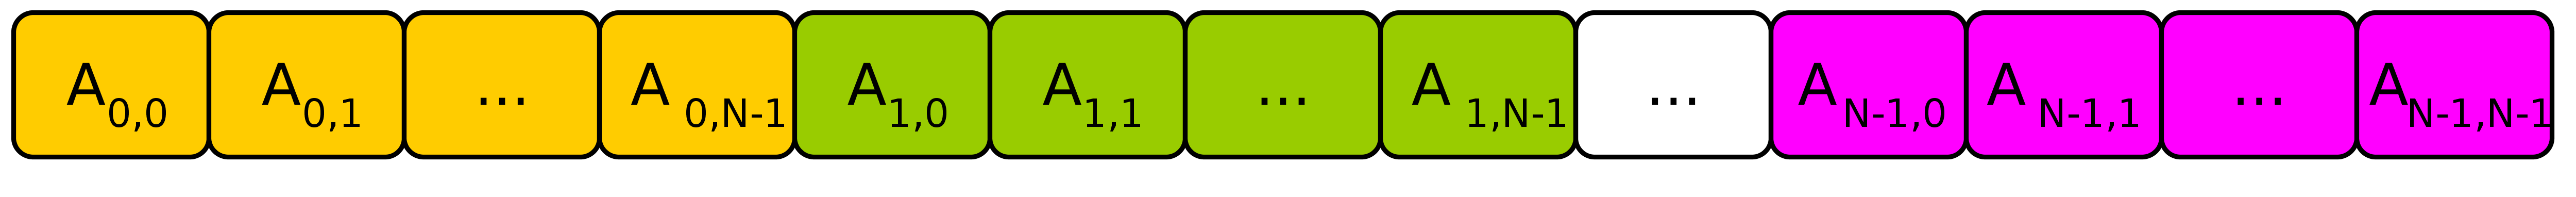
\includegraphics[width=10.5cm]{two_dim_array.png}
        \end{center}
        \begin{block}{Slow}
            \lstinputlisting[numbers=none]{04_two_dim_array_iteration_slow.c}
        \end{block}
        \begin{block}{Fast, sequential}
            \lstinputlisting[numbers=none]{04_two_dim_array_iteration_fast.c}
        \end{block}
    }
\end{frame}
%%%%%%%%%%%%%%%%%%%%%%%%%%%%%%%%%%%%%%%%%%%%%%%%%%%%%%%%%%%%%%%%%%%%%%%%%%%%%%%%%
\begin{frame}{goto statement}
    \note{Eiichi Goto http://en.wikipedia.org/wiki/Eiichi\_Goto}
    \only<1>{
        Edsger Dijkstra (March 1968). \\ "Go To Statement Considered Harmful".
    }
    \only<2>{
        \lstinputlisting{04_no_goto_example.c}
    }
    \only<3>{
        \lstinputlisting{04_goto_example.c}
    }
\end{frame}
%%%%%%%%%%%%%%%%%%%%%%%%%%%%%%%%%%%%%%%%%%%%%%%%%%%%%%%%%%%%%%%%%%%%%%%%%%%%%%%%%
\begin{frame}{Common traps}
    \only<1>{
        \lstinputlisting{04_ifelse_trap.c}
    }
    \only<2>{
        \lstinputlisting{04_switch_trap1.c}
    }
    \only<3>{
        \lstinputlisting{04_if_trap.c}
    }
    \only<4>{
        \lstinputlisting{04_switch_trap2.c}
    }
    \only<5>{
        \lstinputlisting{04_switch_trap3.c}
    }
    \only<6>{
        \lstinputlisting{04_return.c}
    }

\end{frame}
%%%%%%%%%%%%%%%%%%%%%%%%%%%%%%%%%%%%%%%%%%%%%%%%%%%%%%%%%%%%%%%%%%%%%%%%%%%%%%%%%

\end{document}
